\section{Architecture design and implementation}
\subsection{Platforms classification and choice}
For the first version of the test environment and the demonstration of the workflow process and architecture, three types of platforms were distinguished: SaaS, libraries, and containers
\subsubsection{Web Platform}
For web platforms are understood as a remote access point to which public IP address can only assign, this platform also does not have the opportunity to measure the CPU time and Memory KB, it uses only the time of execution of the query or process. In this paper, as an example, the CloudcheckR\cite{cloudcheckr} is used. CloudCheckr provides an associated cost and security management platform for cost management, AWS inventory, continuous security and compliance auditing across your AWS investment. It also provides comprehensive visibility into a user's cloud environment including billing details, resources, multi-accounts, services, configurations, logs, permissions, changes and more.  CloudcheckR is a commercial offer,  for the tests used a free 14-day trial. For Access, it is necessary to create an admin access key, which specified further in the test environment configuration file.
\subsubsection{Libraries}
Libraries are aggregators of several cloud platforms for standardised and straightforward access and management. In this case using the Python library, since the code of the test environment written in this language. For evaluation example, using the previously mentioned Libcloud.  Libcloud is a Python library for interacting with many of the popular cloud service providers using a unified API. It was created to make it easy for developers to build products that work between any of the services that it supports. Compare to other platforms library is the easiest to use and since it runs on the local machine, it is possible to test the performance of the prototyping python process.
\subsubsection{Containers}

\textbf{Composed Containers}
Is the platform that is running with the help of the '\textit{docker compose up}' command and consists of some other containers. As an example used MistIO\cite{mistio} which us managing a mix of public and private clouds, hypervisors, containers, and bare metal trying to optimise costs and policies across platforms also providing visibility and control that makes it easier to govern various infrastructure consistently. Main features are:
\begin{itemize}
    \item Control hybrid environments
    \item Enable self-service
    \item Keep track of usage and cost
    \item Workflows automation
\end{itemize}
Such characteristics as CPU time and Memory KB extracted efficiently through the docker open API.

\textbf{Single Container}
A single container that runs through the \textit{docker run} command, the platform consists of one single image. ManageIQ\cite{manageiq} is a platform that provides one single image. ManageIQ is an open-source Management Platform that delivers the insight, control, and automation that enterprises need to address the challenges of managing hybrid IT environments. It has the following feature sets:
\begin{itemize}
    \item \textbf{Insight}: Discovery, Monitoring, Utilization, Performance, Reporting, Analytics, Chargeback, and Trending.
    \item \textbf{Control}: Security, Compliance, Alerting, Policy-Based Resource and Configuration Management.
    \item \textbf{Automate}: IT Process, Task and Event, Provisioning, Workload Management and Orchestration.
    \item \textbf{Integrate}: Systems Management, Tools and Processes, Event Consoles, CMDB, RBA, and Web Services.
\end{itemize}
As well as with composed containers it is easy through the docker to get access to the characteristics of the CPU time and Memory KB.
\subsection{Architecture approach}
Designed testbed aims to improve quality of research overall and particularly to create such an environment which would create utterly repeatable set of experiments for management platforms specifying  authentication data(credentials, tokens or access keys) with simple YAML file containing instructions in which order, what platforms what amount of times should repeat particular experiments and generate standardised output as raw data, graph or latex table. 

While development process every action which supposed to be evaluated should be described with respect of architecture overall and python decorators which are warping methods. In parallel with the platforms, there is also a set of decorators for defining the method and metrics that extracting from the experiments.
\subsubsection{decorator timing} created for simple time calculation of particular method execution. 
\subsubsection{decorator docker consumption} has an input argument that takes the value of the list of containers, and it will collect the metrics of CPU time and used Memory KB via docker API for each container.
\subsubsection{decorator docker consumption} also collects the use of the CPU time and Memory KB, but unlike the docker, these values are not the container, but the python's process, also this process is determined automatically.
\subsubsection{decorator tagging} this decorator has a double benefit, the first is for the more convenient output of information in the form of a dictionary(json) and further easy parsing. And also for registration and mapping all the methods that use it. In the result, a map of all methods and tags recorded in the global variable, which is necessary for the next steps in the workflow. 
\subsection{Client implementation}
Inside every evaluation client, the method for evaluation should be wrapped by several decorators that are defined above. Each method, regardless of its functionality and classification, has two decorators, the decorator of time should be at the lowest level, so that time is calculated only for the method, and not for other decorators. And the second decorator of the tag, at the highest level, to systematise the output and results of all decorators. When passing a parameter to this decorator, need to be mentioned the correct format to use: '\textit{NameOfProvider:NameOfResource:Action}',  where '*' stands for 'any'. For example '\textit{*:system:start}' means that this method responsible for the start of the system, and '\textit{aws:provider:create}' defines a method for creating an AWS provider. Between this wrappers, can be as many additional decorators. For evaluation of the libcloud created a specially written decorator for the use of resources by the python, while for the Docker-based platforms written a decorator for the docker resource consumption.
\subsection{Workflow}
UML diagrams are presented in the addendum to this work[link to github], here is given the general architecture in Figure \ref{fig}. When the testbed starts, all the methods that are under this directory classes initialised. All methods with their description saved as a map under the global variable. In the future, the configuration file, as well as the matrix, are loaded. The configuration file contains the information necessary for authorisation (for example, a secret key and an access key for Amazon, an access key for the CloudcheckR, etc.). The matrix is designed to simplify and systematise tests and experiments for multiple platforms. For experiment running, matrix file should have a format in the proposed form:
\begin{lstlisting}[language=yaml]
mistio:
  repetitions: 50
  output_dir: /home/ubuntu/experiments
  cmps: [mistio]
  providers: [aws]
  pre_experiment:
    system:
      -start
  post_experiment:
    system:
      -stop
  actions:
    provider:
      - create
      - list
      - delete
\end{lstlisting}
This YAML interpreted as follow: Create an excerpt under the name of "mistio", which will save all the results in the /home/ubuntu/experiments/mistio directory, perform all the experiments only for the mistio platform and for the AWS provider, start the system before the start of the evaluation, and at the end also stop. Do the experiments over the provider (AWS) and create it 50 times, show it, delete it.
\begin{figure}[htbp]
\centerline{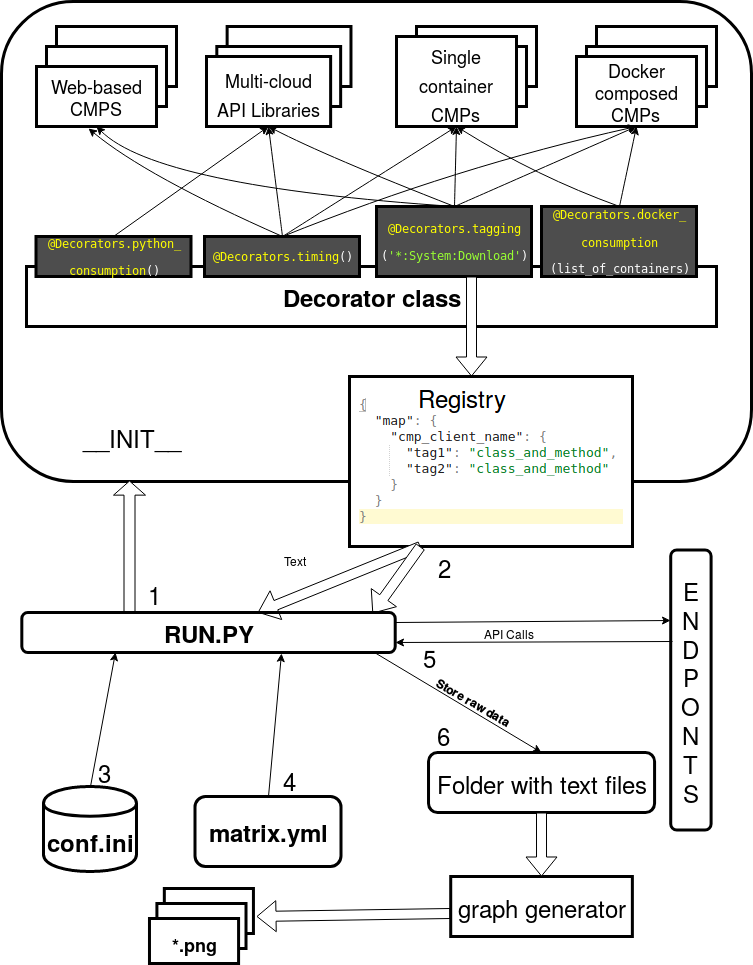
\includegraphics[scale=0.33]{pics/PA1_Diagram.png}}
\caption{Architecture of evaluation application}
\label{fig}
\end{figure}
After reading all the files(configuration and matrix) and creating a common register with the decorator, these data combined and tests produced one by one. Later on, when results are ready, they are dynamically stored in the above folder. In the last step, from the data obtained during the experiment, graphs and matrixes are generated that compare the individual functions.

As it seen the architecture is very flexible and it's easy to add some new platform as well as a characteristic for comparison. With the matrix, it is also possible to create any experiment with the most unusual conditions and the order to evaluate functions and actions